\section{Allgemeine Vorgehensweise}
Im Folgenden wird die allgemeine Vorgehensweise beschrieben. Zur besseren Strukturierung, Dokumentierung und klaren Aufgabenverteilung, haben wir uns ein eigenes GitHub-Repository \footnote{https://github.com/HallerPatrick/AI-Birds-LeveGANerator} aufgesetzt, in welchem ebenfalls die Arbeitszeiten an den bestimmten Issues festgehalten wurden. Die wichtigsten Aufgaben werden in den nachfolgenden Unterkapiteln näher erläutert. [Graphen, allgemeine Struktur]

\begin{figure}
    \centering
    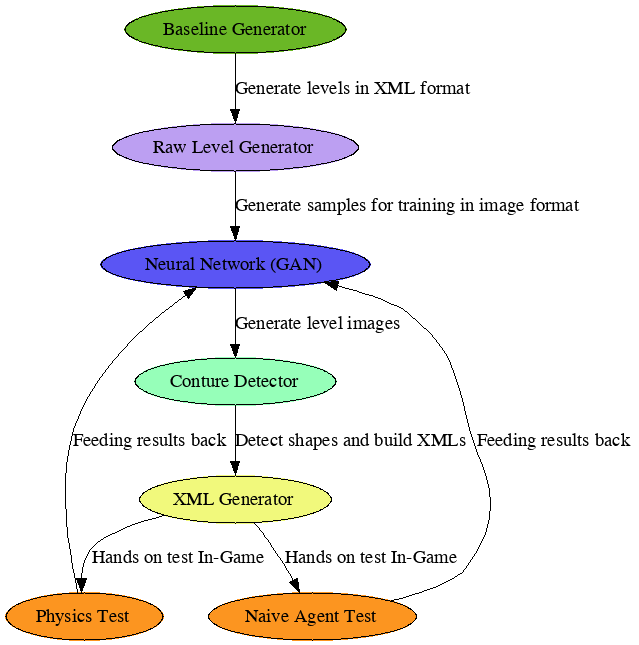
\includegraphics[height=12cm, width=10cm]{img/project_structure.png}
\end{figure}

\subsection{Erkennen der  Konturen von Zentroiden}
...
\subsection{Parsen von XML in JSON}
Zur Generierung der Level war es notwendig, vorhandene Level, welche im JSON-Format codiert wurden, in äquivalente XML-Formate umzuwandeln. Dazu entwickelten wir einen XmlWriter sowie JsonToXmlParser in Python. \\ Der XmlWriter schreibt zunächst den standardisierten Kopf der XML-Dateien, welche die Codierung, die Breite des Levels (hier: 2) sowie die Minimum-/Maximum-Weite der Kamera beinhaltet. Der Parser liest nun die JSON-Datei und schreibt für jeden Block mithilfe der "add"-Methoden des XmlWriters die XML-Datei. Jeder eingelesene Vogel, Block, Schwein etc. wird dabei in seine eigene Liste eingeschrieben (inklusive der Attribute, z.B. "id", "rotation"...). Nach dem Erreichen des Endes der JSON-Datei erfolgt letztendlich der Abschluss des XML-Dokuments, bei welchem das Tag der GameObjects und vom Level geschlossen werden.
\subsection{Automatisierung der Abläufe mithilfe von Powershell unter Windows}
Um zu vermeiden, dass alle Komponenten einzeln und umständlich gestartet werden müssen, haben wir es uns außerdem zur Aufgabe gemacht, ein Automatisierungsskript aufzusetzen, welcher diesen Schritt für uns übernimmt. Als Skriptsprache erschien uns PowerShell am sinnvollsten, da dieses ein fester Bestandteil von Windows 10 (dem gängigsten Betriebssystem) ist und aufgrund dessen keine extra Tools installiert und erläutert werden müssen. \\Das Skript startet zunächst ScienceBirds und skaliert diesen mithilfe von Window-Resizer (Tool zur nutzerbasierten Steuerung der Standardgröße eines Fensters, hier: ScienceBirds) auf einen bestimmten Wert, da der Agent sonst mit der Größe des ScienceBirds-Fensters nicht einverstanden ist. Im Anschluss wird der Agent und der Server automatisch in der Eingabeaufforderung gestartet. Wir konnten beobachten, dass durch den Startklick des Skripts alle benötigten Fenster ordnungsgemäß gestartet wurden und der Agent das Spiel wie erwartet, selbstständig gespielt hat. [Screenshot von GUI]
\subsection{Konvertierung von Pythons Pillow Koordinaten in ein kartesisches XML-Koordinatensystem}
[Patrick]
\subsection{Verdeutlichen der Konturen der erzeugten RAW-Bilder zur besseren Erkennung vor Training}
Der Konturen-Erkenner hatte in unserem Durchlauf Probleme, die Umrisse der erzeugten Zentroide zu erkennen. Aufgrund dessen mussten wir die Konturen, welche erzeugt werden, vor dem Beginn des Trainings verstärken, damit diese eindeutig von unserem Erkenner gefasst werden können. \\
\begin{figure}
	\centering
	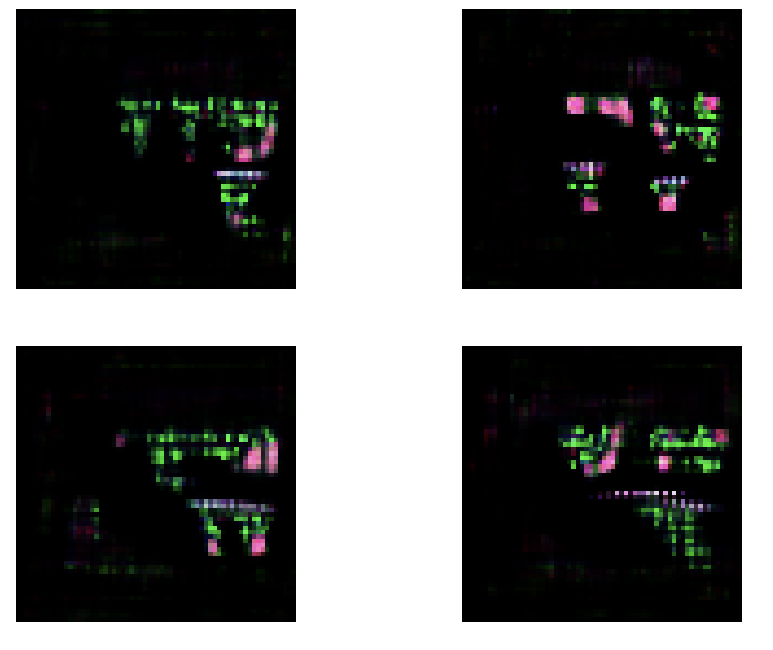
\includegraphics[height=10cm, width=10cm]{img/blurry_attempts.png}
	\caption{Verschwommene Konturen führen zu Problemen bei der Erkennung}
\end{figure}
\subsection{Aufsetzen eines Re-Evaluierungssystems}
[Patrick]